%% Miscellaneous
%
%
%\documentclass{article}
%
%\usepackage{fancyhdr}
%\usepackage{extramarks}
%\usepackage{amsmath}
%\usepackage{amsthm}
%\usepackage{amsfonts}
%\usepackage{tikz}
%\usepackage{enumerate}
%\usepackage{graphicx}
%\graphicspath{ {images/} }
%\usepackage[plain]{algorithm}
%\usepackage{algpseudocode}
%\usepackage[document]{ragged2e}
%\usepackage{textcomp}
%\usepackage{color}   %May be necessary if you want to color links
%\usepackage{import}
%\usepackage{hyperref}
%\hypersetup{
%    colorlinks=true, %set true if you want colored links
%    linktoc=all,     %set to all if you want both sections and subsections linked
%    linkcolor=black,  %choose some color if you want links to stand out
%}
%
%\usetikzlibrary{automata,positioning}
%
%
%% Basic Document Settings
%
%
%\topmargin=-0.45in
%\evensidemargin=0in
%\oddsidemargin=0in
%\textwidth=6.5in
%\textheight=9.0in
%\headsep=0.25in
%\setlength{\parskip}{1em}
%
%\linespread{1.1}
%
%\pagestyle{fancy}
%\lhead{\hmwkAuthorName}
%\lfoot{\lastxmark}
%\cfoot{\thepage}
%
%\renewcommand\headrulewidth{0.4pt}
%\renewcommand\footrulewidth{0.4pt}
%
%\setlength\parindent{0pt}
%
%
%\newcommand{\hmwkTitle}{Math Review Notes---Miscellaneous}
%\newcommand{\hmwkAuthorName}{\textbf{G. Faletto} }
%
%
%%%%%% Title Page
%
%
%\title{
%    \vspace{2in}
%    \textmd{\textbf{ \hmwkTitle}}\\
%}
%
%\author{Gregory Faletto}
%\date{}
%
%\renewcommand{\part}[1]{\textbf{\large Part \Alph{partCounter}}\stepcounter{partCounter}\\}
%
%
%%%%%% Various Helper Commands
%
%
%%%%%% Useful for algorithms
%\newcommand{\alg}[1]{\textsc{\bfseries \footnotesize #1}}
%
%%%%%% For derivatives
%\newcommand{\deriv}[2]{\frac{\mathrm{d} #1}{\mathrm{d} #2}}
%
%%%%%% For partial derivatives
%\newcommand{\pderiv}[2]{\frac{\partial #1}{\partial #2}}
%
%%%%%% Integral dx
%\newcommand{\dx}{\mathrm{d}x}
%
%%%%%% Alias for the Solution section header
%\newcommand{\solution}{\textbf{\large Solution}}
%
%%%%%% Probability commands: Expectation, Variance, Covariance, Bias
%\newcommand{\E}{\mathbb{E}}
%\newcommand{\Var}{\mathrm{Var}}
%\newcommand{\Cov}{\mathrm{Cov}}
%\newcommand{\Bias}{\mathrm{Bias}}
%\newcommand\indep{\protect\mathpalette{\protect\independenT}{\perp}}
%\def\independenT#1#2{\mathrel{\rlap{$#1#2$}\mkern2mu{#1#2}}}
%\DeclareMathOperator{\Tr}{Tr}
%
%\theoremstyle{definition}
%\newtheorem{theorem}{Theorem}
%\theoremstyle{definition}
%\newtheorem{proposition}[theorem]{Proposition}
%\theoremstyle{definition}
%\newtheorem{lemma}[theorem]{Lemma}
%\theoremstyle{definition}
%\newtheorem{corollary}{Corollary}[theorem]
%\theoremstyle{definition}
%\newtheorem{definition}{Definition}[section]
%\newtheorem*{remark}{Remark}
%\theoremstyle{definition}
%\newtheorem{exercise}{Exercise}
%\theoremstyle{definition}
%\newtheorem{example}{Example}[section]
%
%%%%%% Tilde
%\newcommand{\textapprox}{\raisebox{0.5ex}{\texttildelow}}
%
%\begin{document}
%
%\maketitle
%
%\pagebreak
%
%\tableofcontents
%
%\
%
%\
%
%\begin{center}
%Last updated \today
%\end{center}
%
%
%
%\newpage
%%
%%%
%%%
%%%
%%%
%%%
%%%
%%%
%%%
%%%%
%%%% Miscellaneous




\chapter{Miscellaneous}

\section{Set Theory}

\begin{proposition}[\textbf{Math 541A Homework Problem}] Let $A,B,\Omega$ be sets.  Let $u:\Omega\to A$ and let $t:\Omega\to B$.  Assume that, for every $x,y\in\Omega$, if $u(x)=u(y)$, then $t(x)=t(y)$.  Show that there exists a function $s: A\to B$ such that
$$t=s(u).$$

\end{proposition}

\begin{proof}
Let \(B' \subseteq B\) be the image of \(\Omega\) under \(t\) (so that \(t\) is surjective onto \(B'\)). Fix \(x \in \Omega\) and let \(y \in \Omega\) range over \(\{\Omega \setminus x \}\). Let \(Y \subseteq \Omega\) be the set of values such that \(t(y) = t(x)\) for all \(y \in Y\). Then let \(s\) map \(u(y) \in A\) to \(t(y) = t(x) \in B\) for every \(y \in Y\). 

\

(Note that if \(x\) is not the only value in \(\Omega\) that \(t\) maps to \(t(x)\), then \(Y\) contains elements other than \(x\); otherwise, \(Y = \{x\}\). In either case this mapping is fine. Note that \(u(y_1)\) does not necessarily equal \(u(y_2)\) for every \(y_1 \neq y_2 \in Y\), but again this does not pose any difficulties for the mapping.)
 
 \
 
 Since this argument is true for every \(x \in \Omega\), we can argue by contradiction that \(s\) is surjective onto \(B'\). Let \(A' \subseteq A\) be the image of \(\Omega\) under \(u\) (so that \(u\) is surjective onto \(A'\)). Suppose there is some \(b \in B'\) such that there is no unused \(a \in A'\) to correspond to it. That is, there are some \(y, z \in \Omega\) such that \(t(z) \neq t(y)\) but \(u(z) = u(y)\). In that case the mapping \(s\) would map \(u(z)\) and \(u(y)\) both to the same value in \(B'\), so one of the values \(t(z)\) or \(t(y)\) would necessarily be missed. But by assumption there is no \(z \in \Omega\) such that \(t(z) \neq t(y)\) but \(u(z) = u(y)\). (Note the contrapositive of the assumption: ``for every $x,y\in\Omega$, if \(t(x) \neq t(y)\), then \(u(x) \neq u(y)\).")
 
 \end{proof}
 
 \begin{remark}By showing this mapping exists, we have shown that the cardinality of \(B'\) is less than or equal to the cardinality of \(A'\).

\end{remark}

\section{Other}

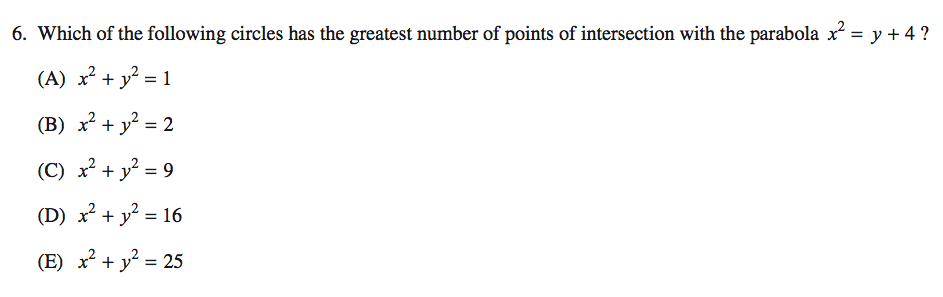
\includegraphics[scale=0.5]{0568_6}

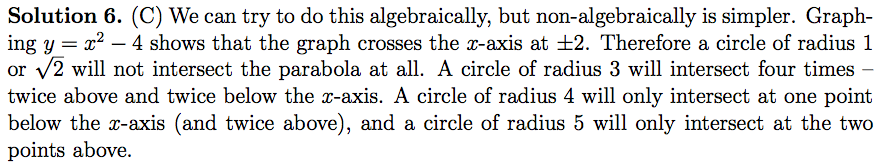
\includegraphics[scale=0.5]{0568_6s}

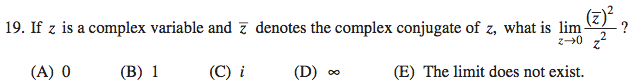
\includegraphics[scale=0.65]{1268_19}

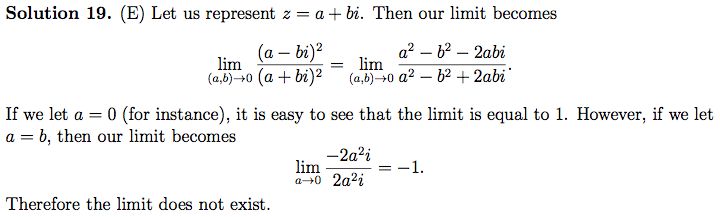
\includegraphics[scale=0.65]{1268_19s}

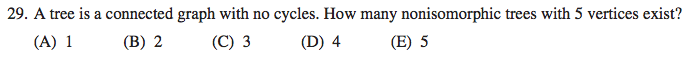
\includegraphics[scale=0.65]{1268_28}

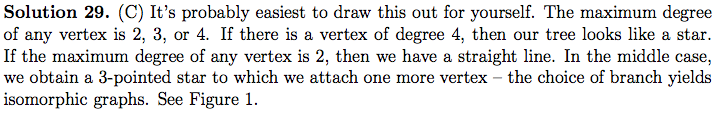
\includegraphics[scale=0.65]{1268_28s}

\begin{center}
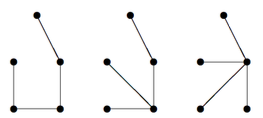
\includegraphics[scale=0.65]{1268_28fig}
\end{center}

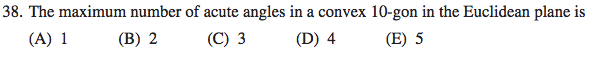
\includegraphics[scale=0.65]{1268_38}

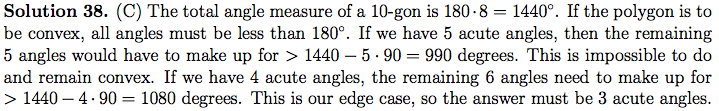
\includegraphics[scale=0.65]{1268_38s}

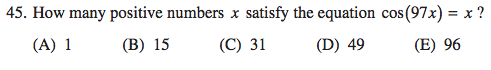
\includegraphics[scale=0.65]{1268_45}

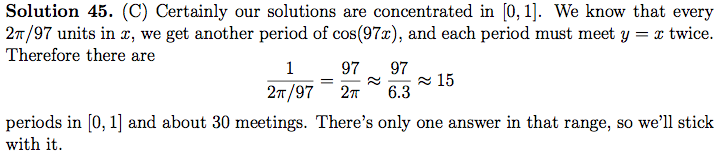
\includegraphics[scale=0.65]{1268_45s}




%\end{document}



